\documentclass[../main.tex]{subfiles}

\begin{document}

\label{app::manual_instalacion}
\subsection{Manual de instalación del proyecto}
En primer lugar, debemos de asegurarnos de tener instalado NodeJS\footnote{\url{ https://nodejs.org/en/download/}} en la máquina en la que vaya a ser ejecutado el proyecto, ya sea un ordenador personal o en un servidor con exposición directa a internet.

Una vez la instalación del entorno de ejecución esté lista, procedemos a descargar el código fuente del proyecto. En este caso, este se encuentra guardado en un repositorio \textit{git} privado, por lo que se necesitará permisos de colaborador para poder acceder a él. 

\begin{lstlisting}[language=bash]
  $ git clone https://github.com/DavidGomez-coder/TFG.git
\end{lstlisting}

A continuación, debemos de abrir una consola de comandos y situarnos en el directorio raíz del proyecto, para instalar así todas las dependencias necesarias. 

\begin{lstlisting}[language=bash]
  $ npm install
\end{lstlisting}

Cuando este proceso finalice iniciamos el proceso de la aplicación ejecutando el siguiente comando:

\begin{lstlisting}[language=bash]
  $ npm start
\end{lstlisting}

, tras el cuál se abrirá en una nueva pestaña del navegador web por defecto en la dirección \url{http://localhost:3000/TFG}; o si estamos utilizando un entorno de servidor, este se podrá acceder sustituyendo \textit{localhost} por la dirección IP de la máquina en cuestión.



\subsection{Manual de usuario de la aplicación}
Lo primero que vemos al iniciar la aplicación, es la siguiente interfaz presentada en la figura \ref{fig::interfaz-usuario}, en la que podemos distinguir claramente una división en dos de la misma, teniendo en la parte superior un panel de navegación que nos permite cambiar entre las dos simulaciones y una parte central con el contenido principal. \\

\begin{figure}[!ht]
  \centering
  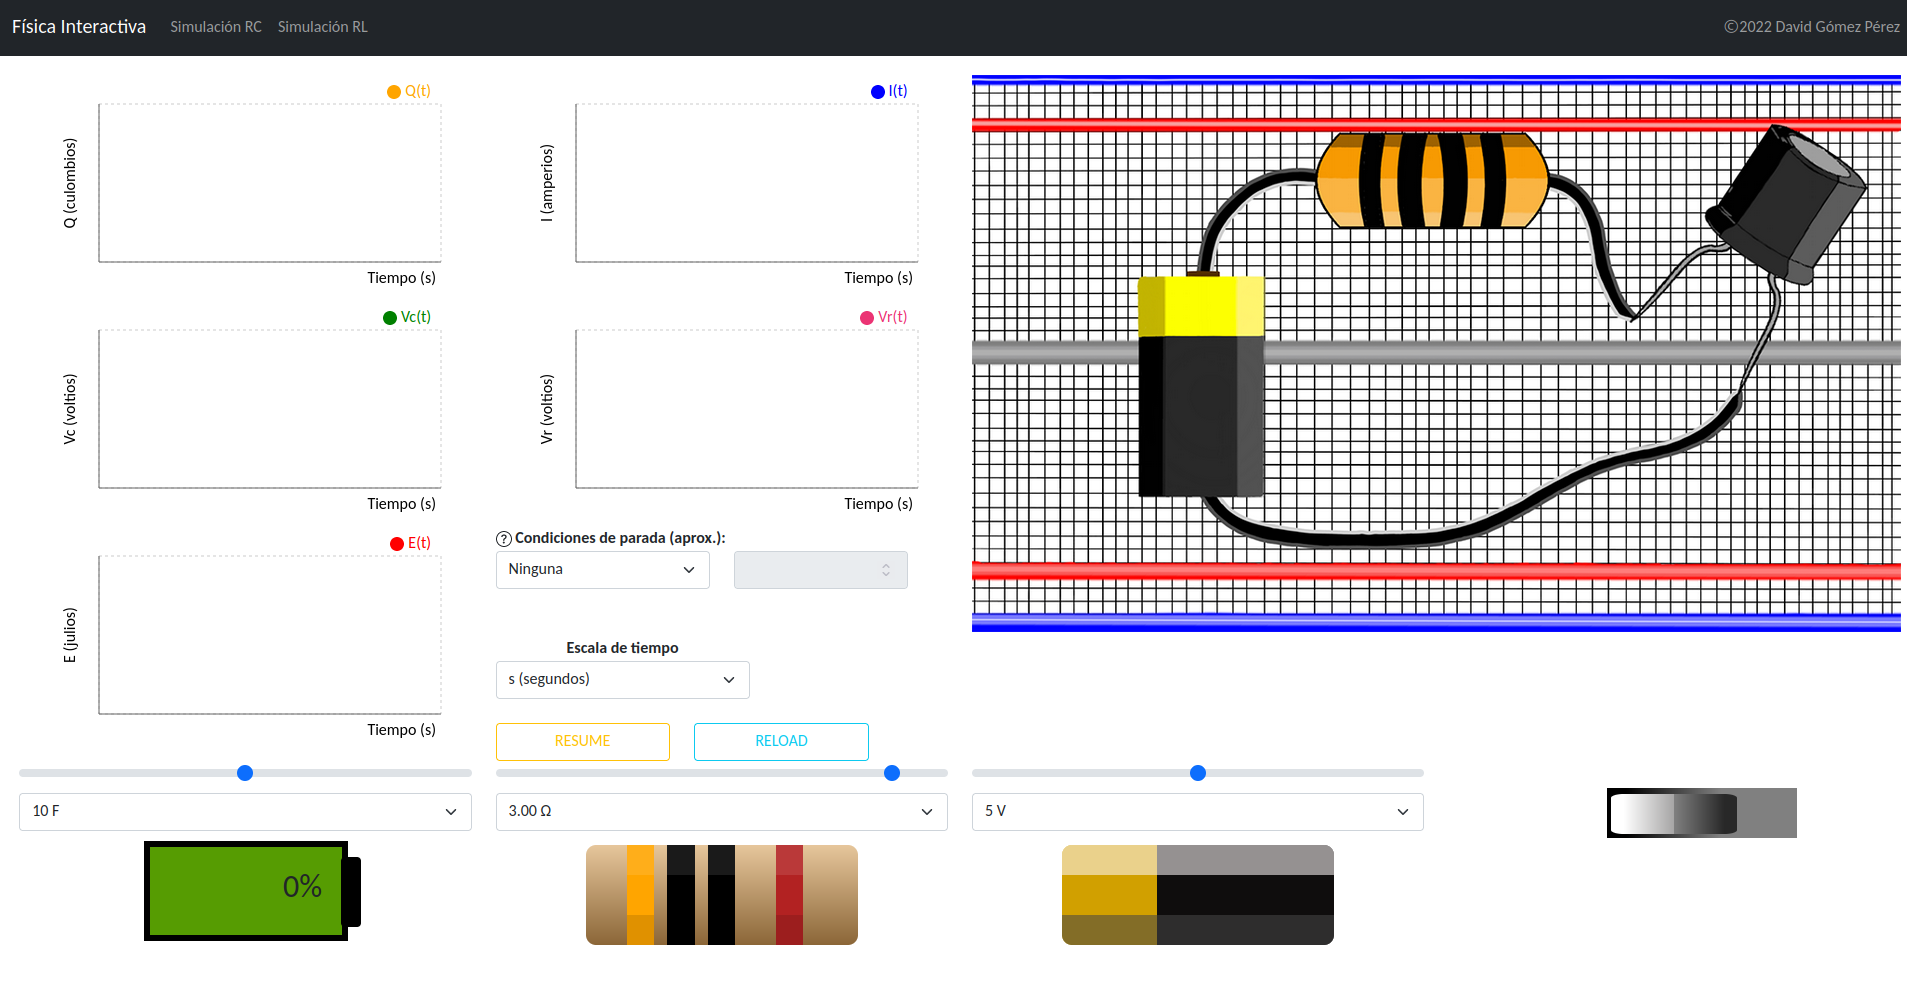
\includegraphics[width=0.85\textwidth]{images/interfaz-usuario.png}
  \caption{Interfaz de usuario de la aplicación (I).}
  \label{fig::interfaz-usuario}
\end{figure}


Para poder diferenciar entre ambos circuitos y saber qué está ocurriendo, se añade una imagen de los mismos sobre el que aparecerán electrones en movimiento, ilustrando así el proceso que está ocurriendo durante la simulación (figura \ref{fig::interfaz-usuario2}). Además, para los estados de disipación de energía, a la fuente se le da cierta transparencia, para emular de alguna manera que esta ha sido quitada del circuito. \\

\begin{figure}[!ht]
  \centering
  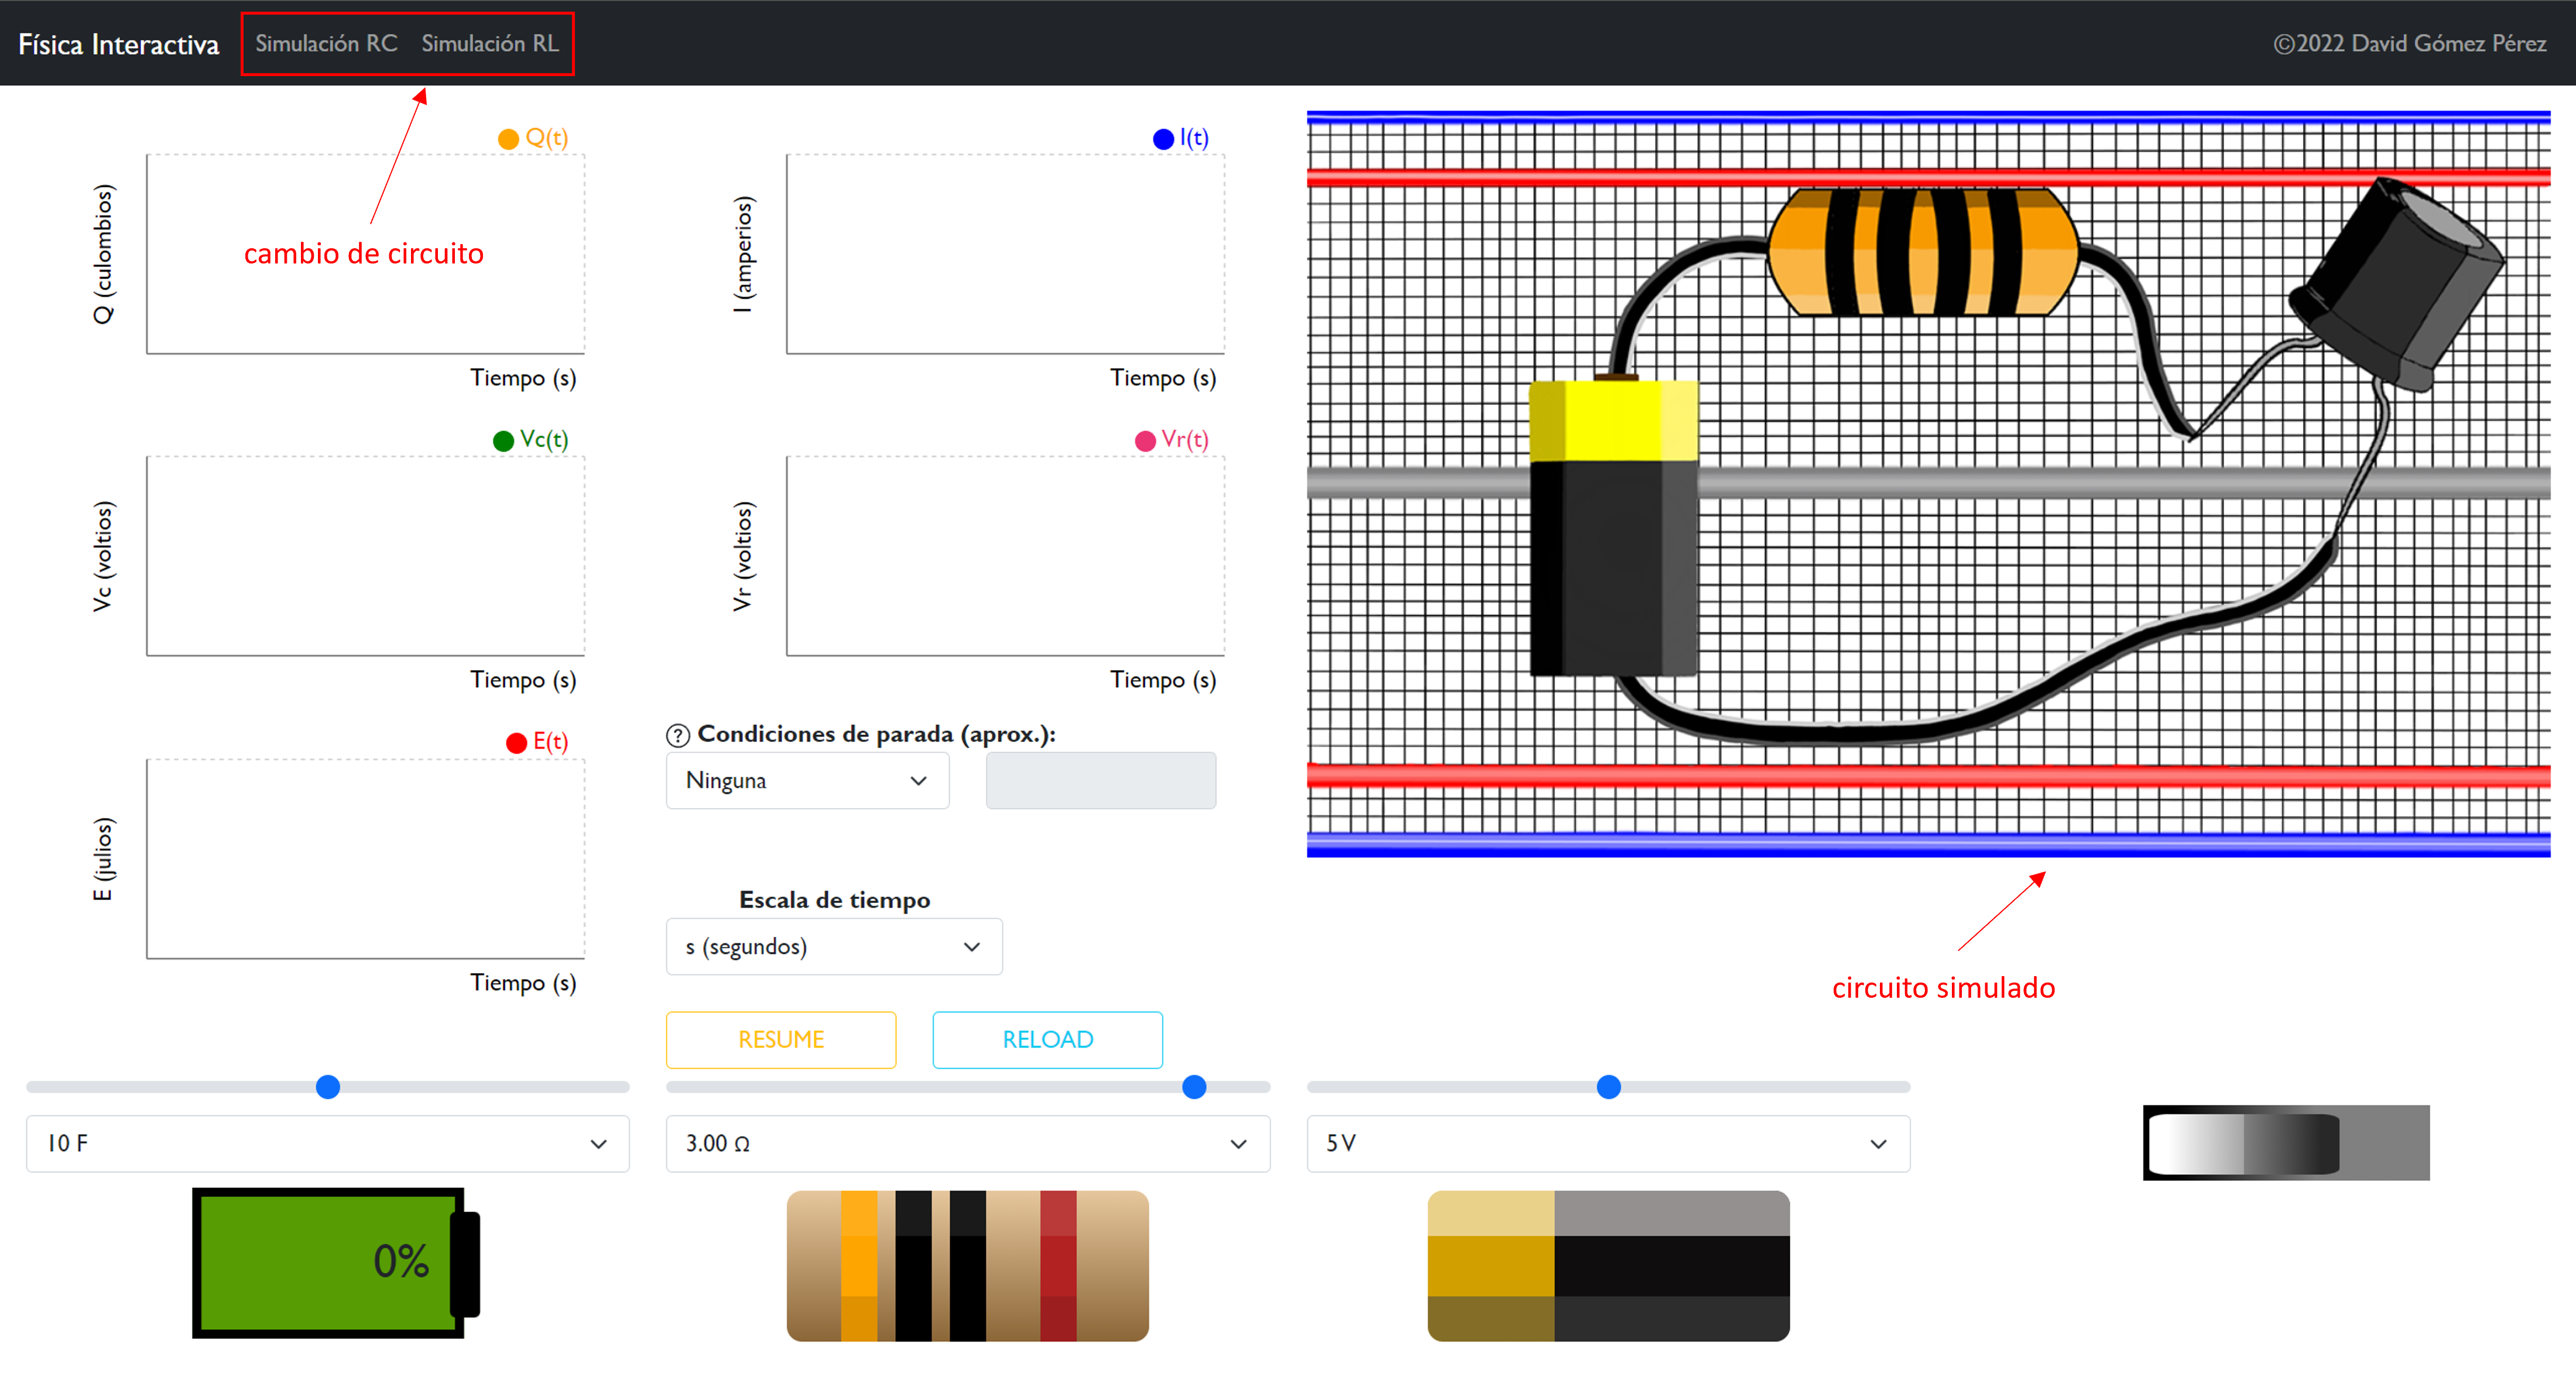
\includegraphics[width=0.85\textwidth]{images/circuito-simulado.png}
  \caption{Interfaz de usuario de la aplicación (II).}
  \label{fig::interfaz-usuario2}
\end{figure}

Junto a la representación del circuito, tenemos la sección dónde se van a mostrar los resultados de cada una de las magnitudes físicas, por las que si pasamos el cursor podremos ver con más en detalle los valores que estas toman (figura \ref{fig::interfaz-usuario3}) .\\

\begin{figure}[!ht]
  \centering
  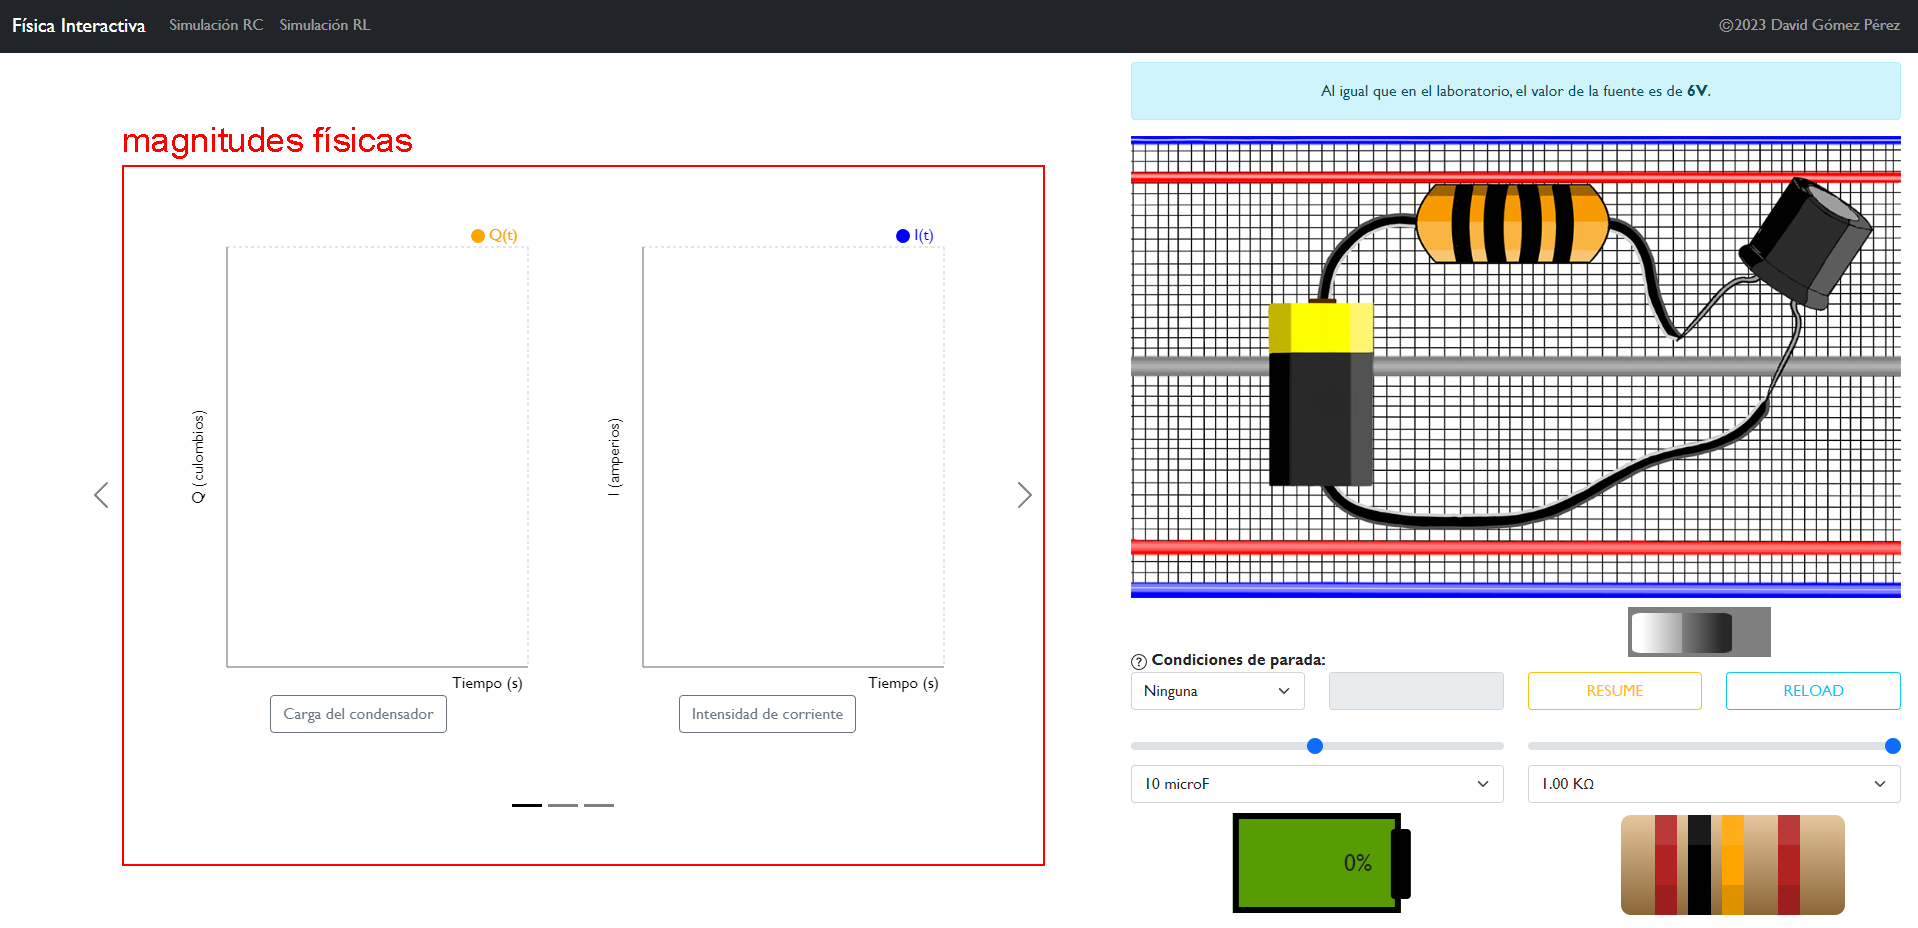
\includegraphics[width=0.85\textwidth]{images/resultados.png}
  \caption{Interfaz de usuario de la aplicación (III).}
  \label{fig::interfaz-usuario3}
\end{figure}

Bajo el circuito, tenemos los controladores de la simulación. Por un lado en la parte superior se encuentra el controlador de las condiciones de parada, las cuáles se encuentran en un \textit{dropdown} (lista desplegable) junto a un \textit{input} que toma el valor de dicha condición.

A su derecha, se encuentran dos botones cuyo objetivo es controlar el estado de la simulación. El botón de la derecha se encarga de reiniciar la simulación (\textit{reload}) y el de la izquierda parar o reanudar esta simulación, dependiendo del estado actual de la misma (figura \ref{fig::interfaz-usuario4.1} y \ref{fig::interfaz-usuario4.2}). \\

\begin{figure}[!ht]
  \centering
  \subfloat[]{
      \label{fig::interfaz-usuario4.1}
      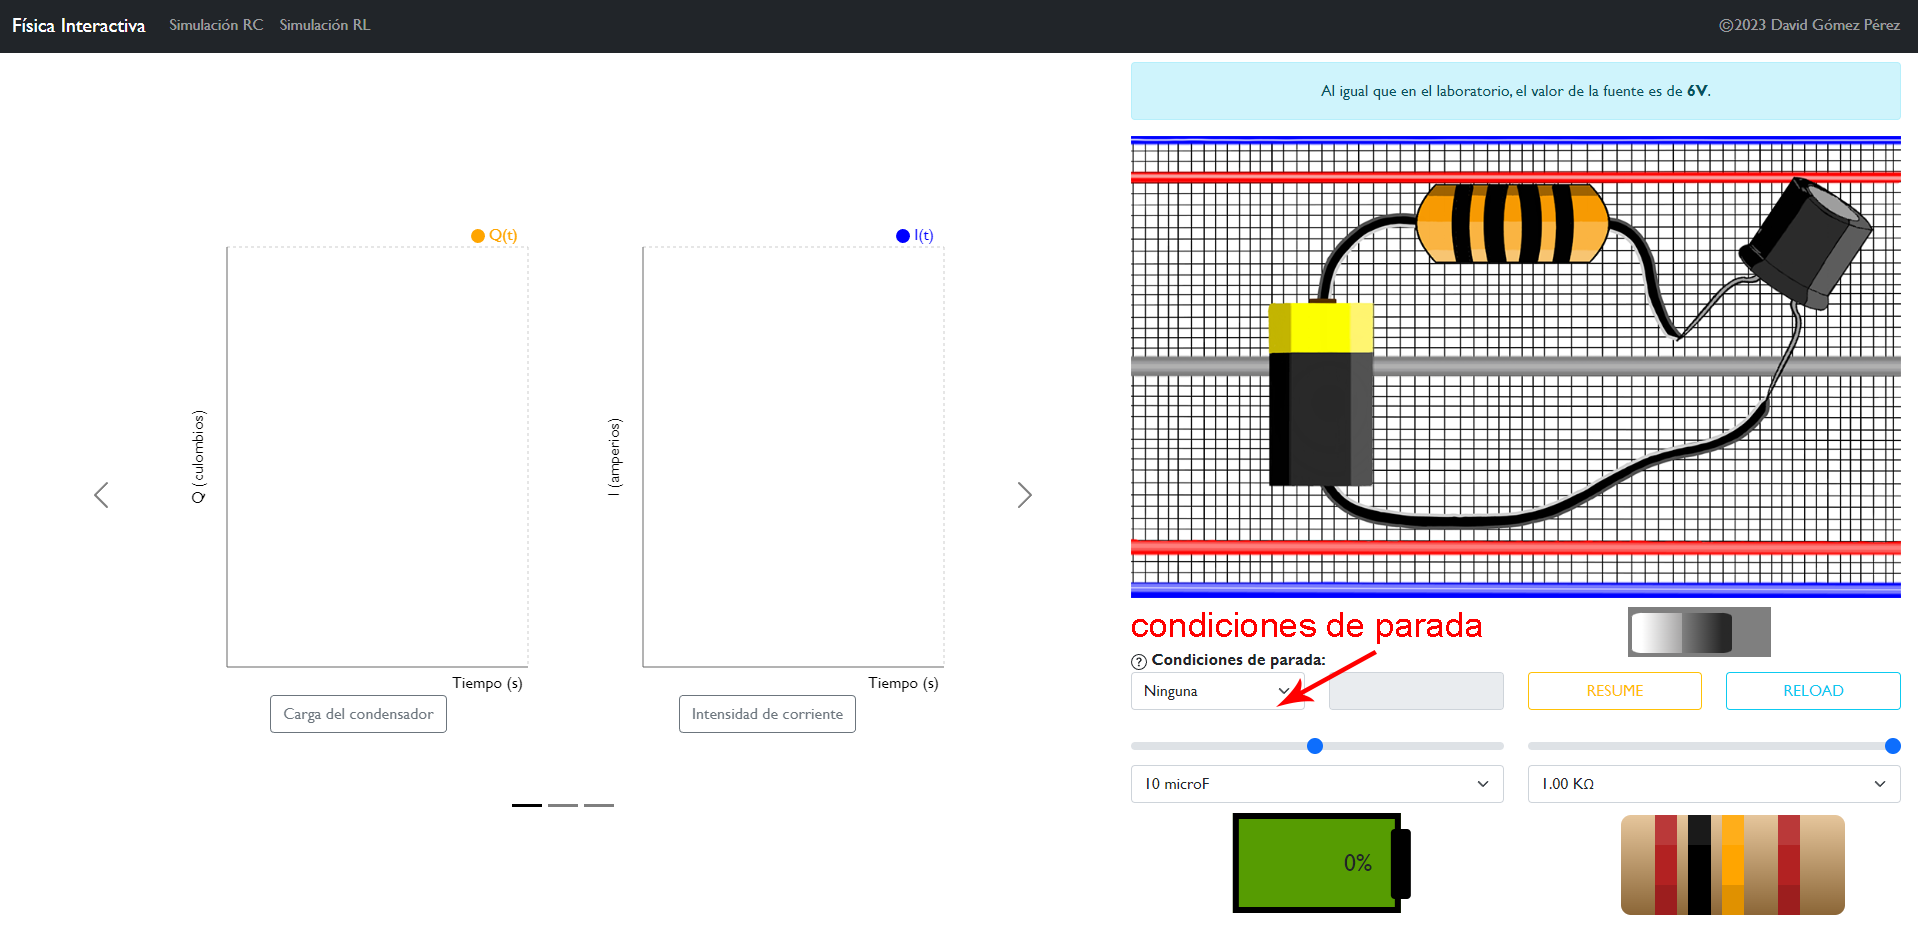
\includegraphics[width=0.85\textwidth]{images/condiciones-escala.png}
  }
  \quad
  \subfloat[]{
      \label{fig::interfaz-usuario4.2}
      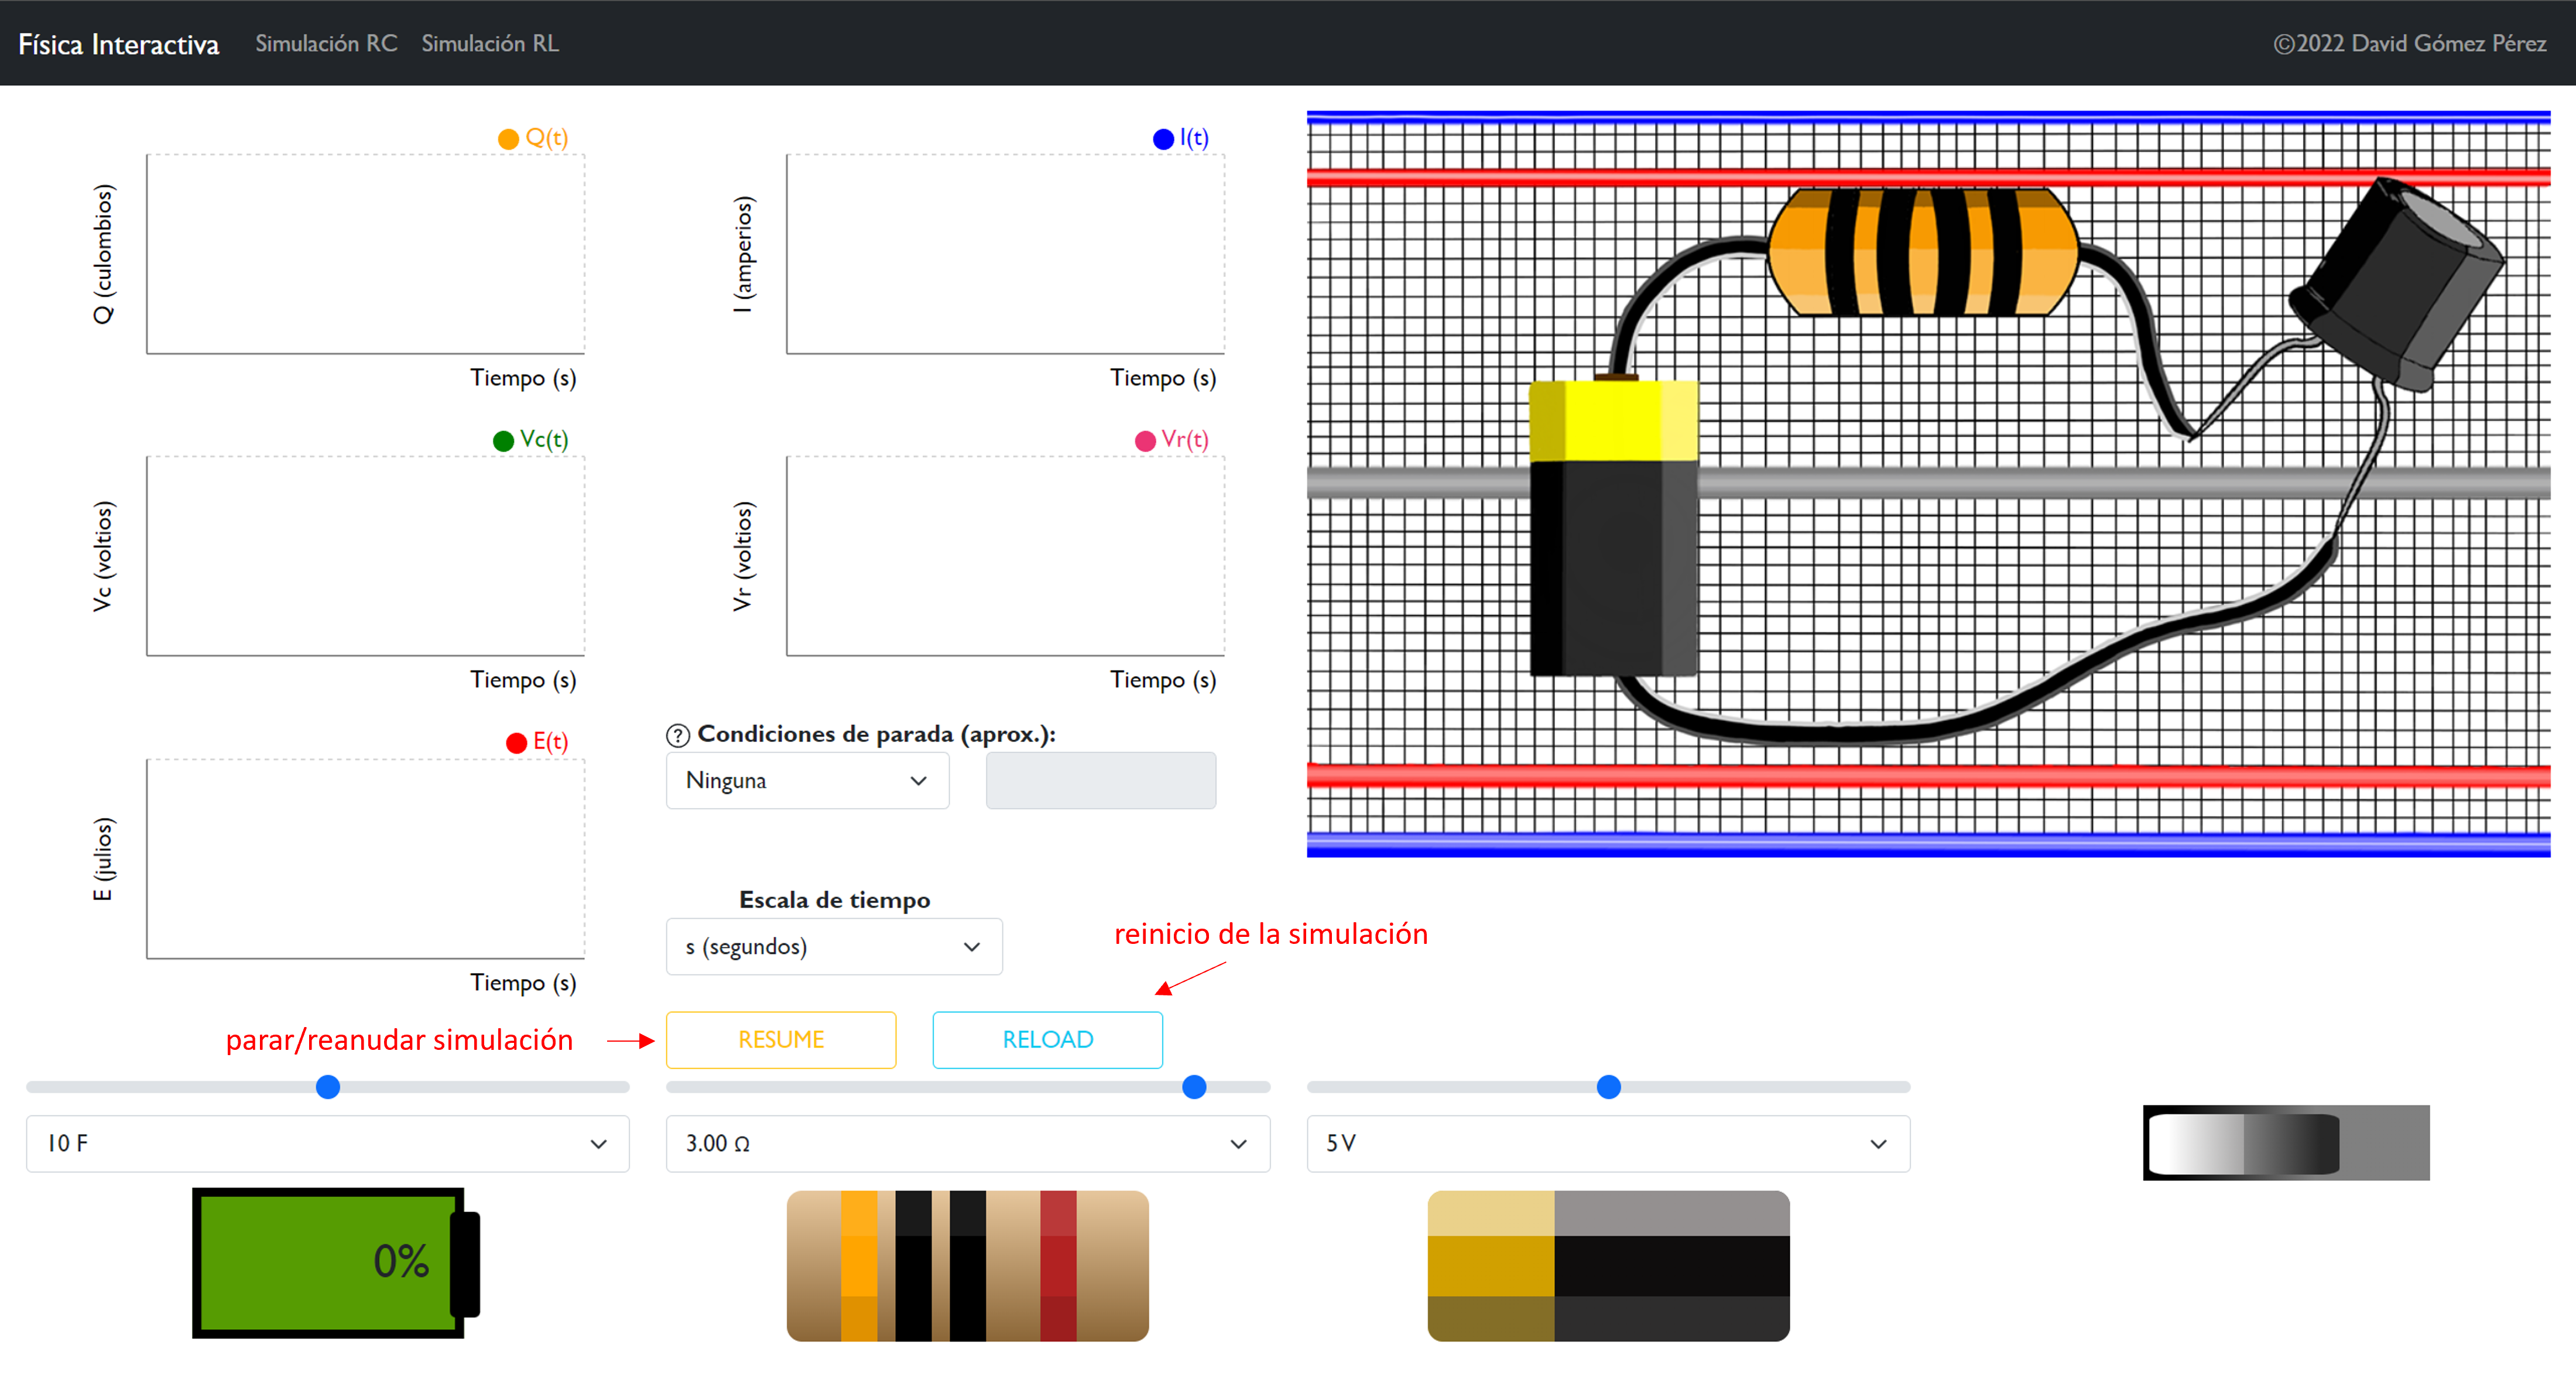
\includegraphics[width=0.85\textwidth]{images/botones.png}
  }


  \caption{Interfaz de usuario de la aplicación (IV).}
  \label{fig::interfaz-usuario4}

\end{figure}


En la parte inferior tenemos los controladores que permiten cambiar los componentes del circuito. Estos se dividen en dos partes. La primera se trata de un \textit{slider} para proporcionar el valor númerico de los mismos mientras que la segunda, situdada justo debajo, es un \textit{dropdown} utilizado para cambiar el multiplicador (por ejemplo, para utilizar una resistencia en mega-ohmios). \\ 

\begin{figure}[!ht]
  \centering
  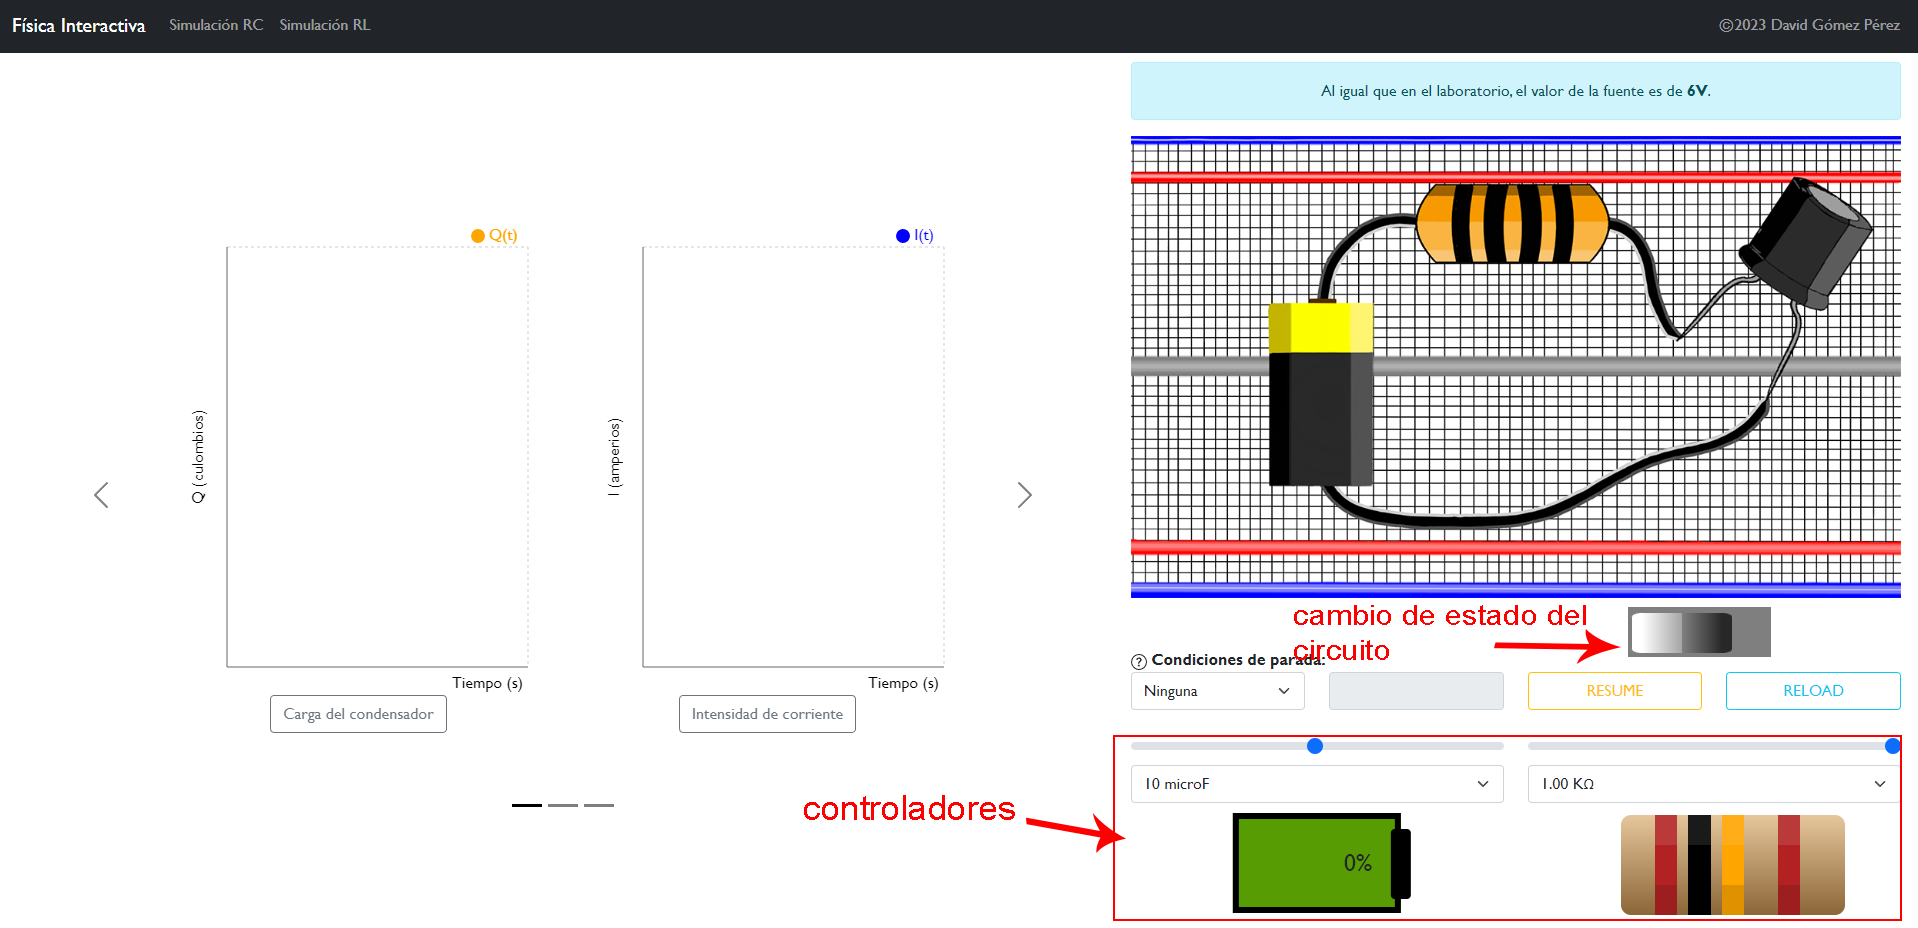
\includegraphics[width=0.85\textwidth]{images/controladores.png}
  \caption{Interfaz de usuario de la aplicación (V).}
  \label{fig::interfaz-usuario5}
\end{figure}

Por último nos quedan los apartados teóricos con información acerca del circuito. Estos se encuentran ocultos, y para activarlos, debemos de pulsar sobre el botón que hay bajo cada una de las magnitudes físicas del panel central. 

\begin{figure}[!ht]
  \centering
  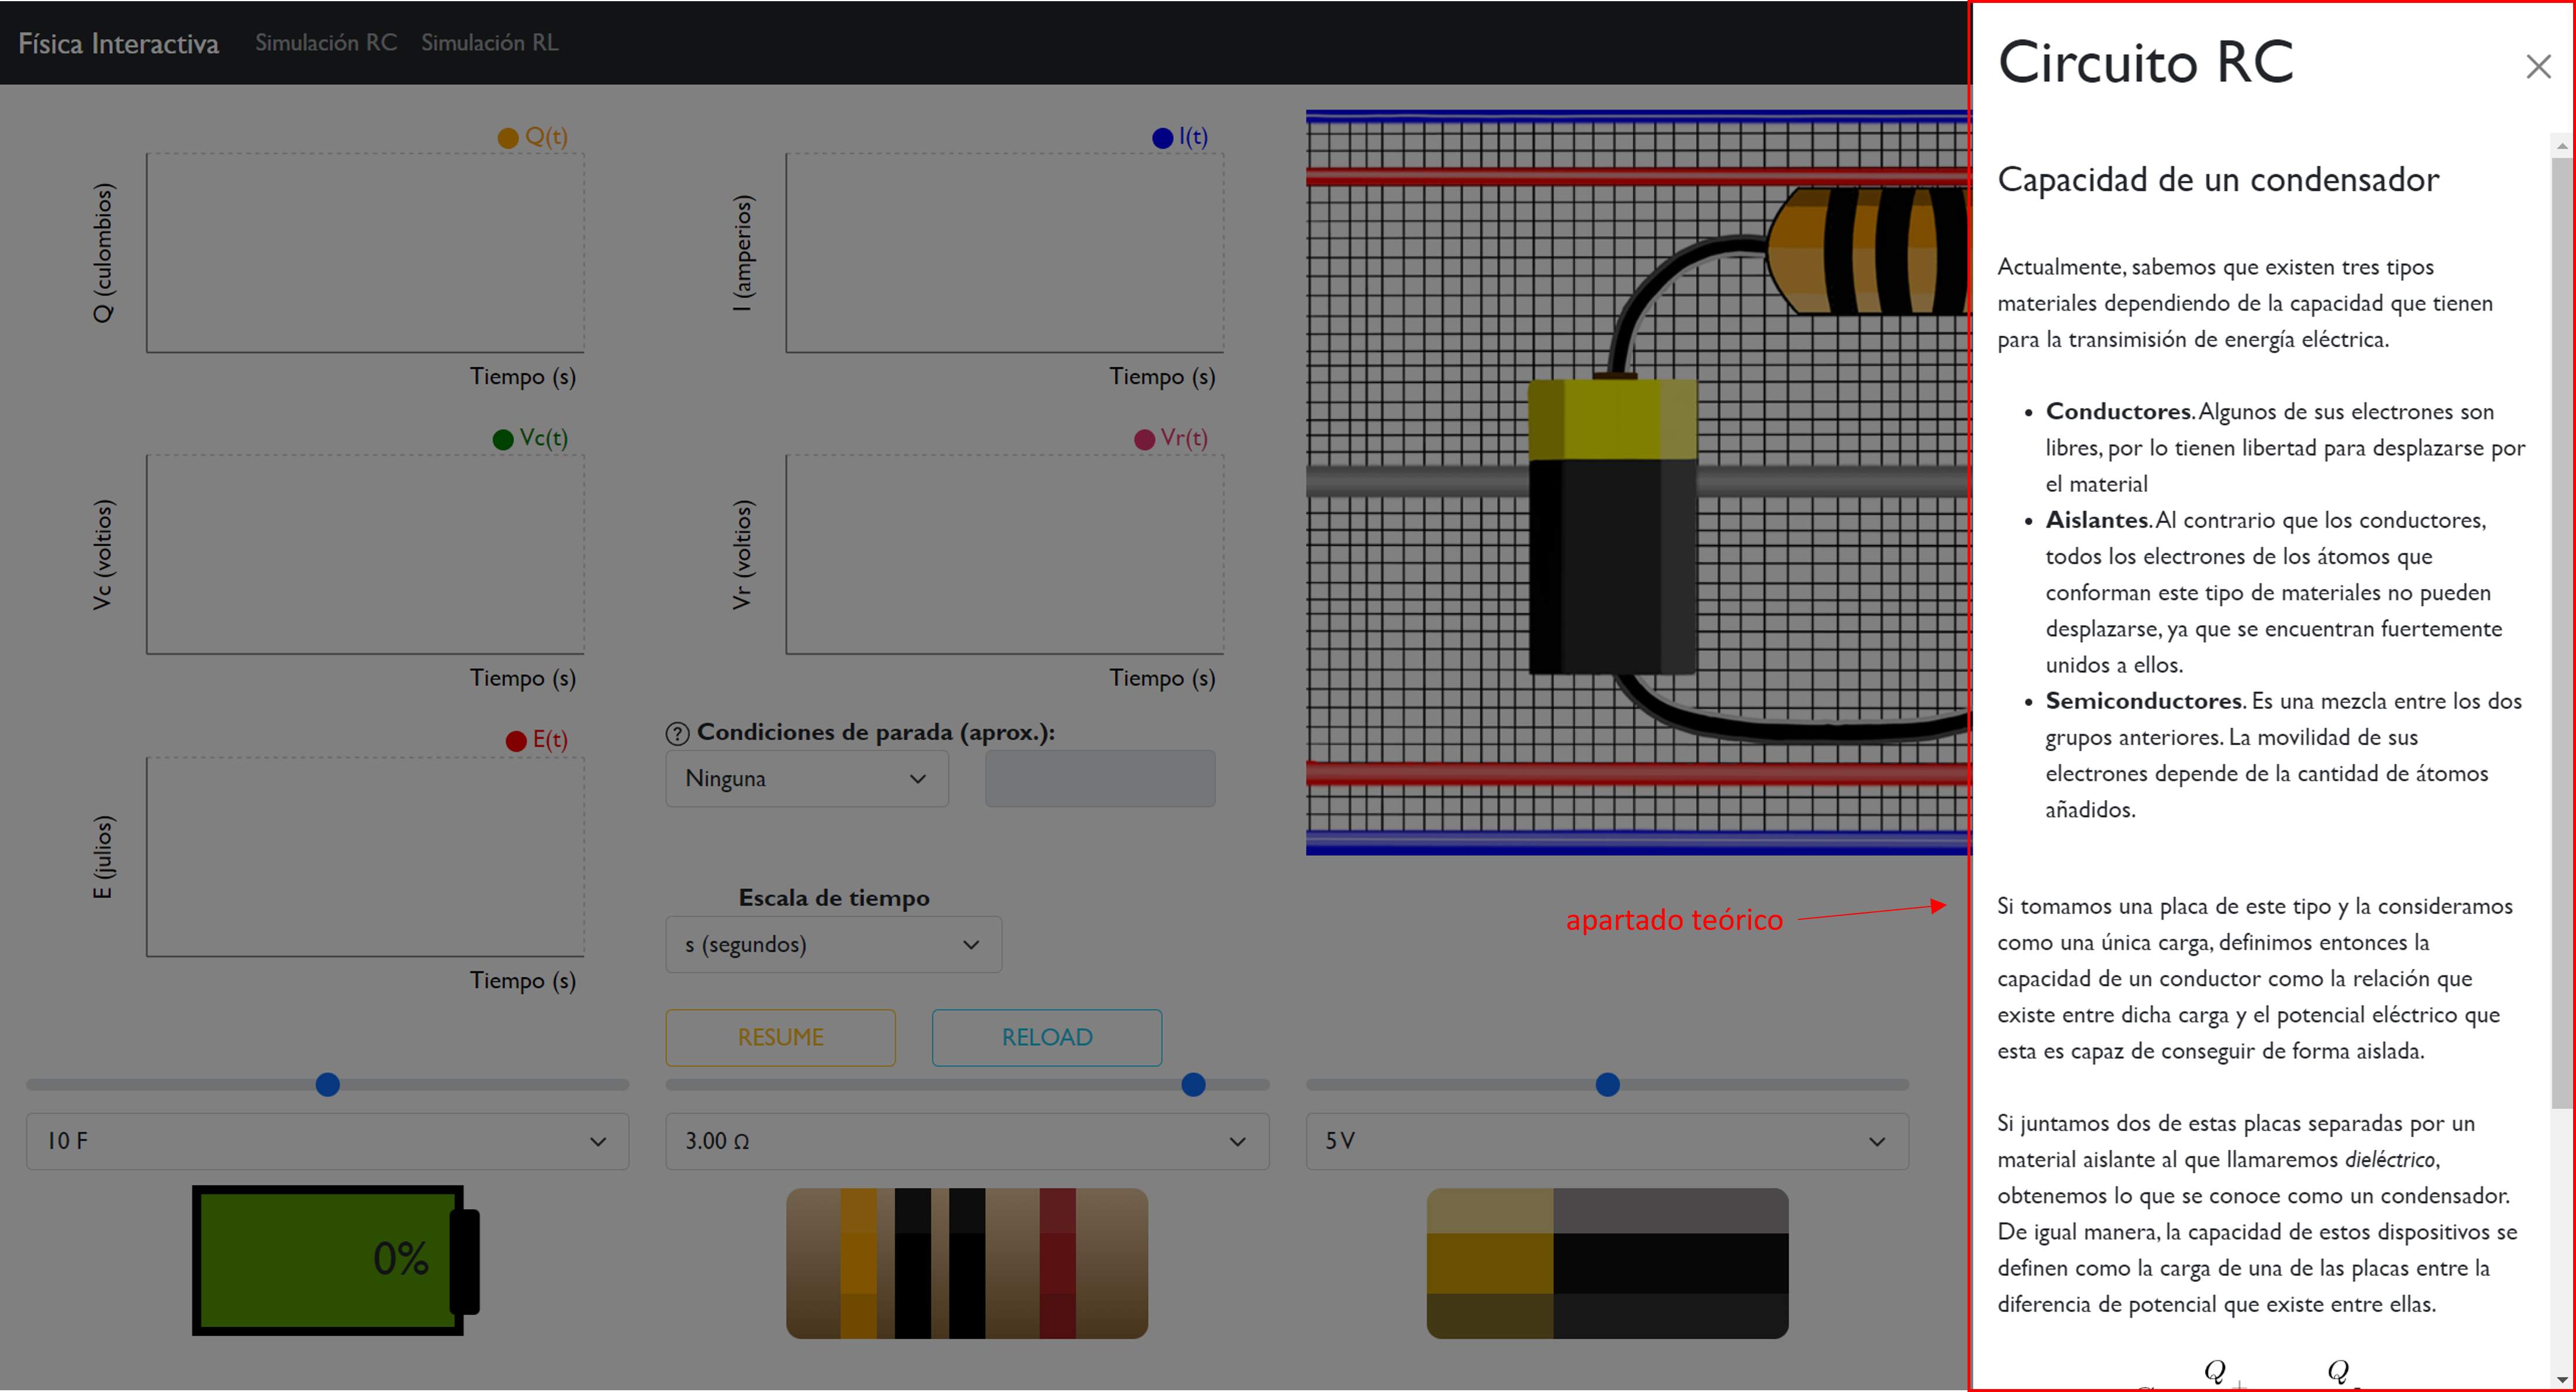
\includegraphics[width=0.85\textwidth]{images/teorico.png}
  \caption{Interfaz de usuario de la aplicación (VI).}
  \label{fig::interfaz-usuario6}
\end{figure}


\subsection{Manual de usuario del script \textit{python} utilizado para las pruebas}
Para utilizar el \textit{script} debemos de  abrir el directorio \textit{simulation-tests} situado en la carpeta raíz del proyecto. El primer paso a realizar es instalar las dependencias guardadas en el fichero \textit{requirements.txt}:

\begin{lstlisting}[language=bash]
  $ pip install -r requirements.txt
\end{lstlisting}

A continuación, podemos utilizar el script de la siguiente manera:

\begin{lstlisting}[language=bash]
  $ python3 main.py [arguments]
\end{lstlisting}

, dónde los argumentos son los que siguen:

\begin{longtable}{|| p{0.2\linewidth} | p{0.2\linewidth} |  p{0.55\linewidth} ||}
  \hline
  
  \textbf{COMANDO} & \textbf{ABREV.} & \textbf{DESCRIPCIÓN} \\ \hline
  --time & -t & Establece la duración de la simulación.  \\ \hline

  --simulationType & -st & Tipo de simulación. Puede tomar los valores ``RC'' o ``RL''. Su definición es obligatoria. \\ \hline

  --incrementValue & -inc & Escala de tiempo para el cálculo de los resultados. Por defecto su valor es de 0.001 segundos. \\ \hline

  --capacitor & -c & Valor en Faradios de la capacidad del condensador. Solo es utilizado cuando el tipo del circuito a simular es RC. Por defecto su valor es de 0.005F. \\ \hline

  --inductor & -i & Valor en Henrios de la inductancia de la bobina. Solo es utilizado cuando el tipo del circuito a simular es RL. Por defecto su valor es de 10H. \\ \hline

  --resistor & -r & Valor en Ohmios de la resistencia. Por defecto su valor es de $3\Omega$. \\ \hline

  --voltage & -v & Valor en Voltios de la fuente de alimentación. Por defecto su valor es de 5V. \\ \hline

  --conditionVal & -condV & Establece la condición de parada de la simulación. Si el circuito a simular es del tipo RC, este valor hará referencia a la carga del condensador. En caso del circuito RL a la intensidad de corriente. \textbf{*} \\ \hline

  --conditionPer & -condP & Establece la condición de parada de la simulación. Si el circuito a simular es del tipo RC, este valor hará referencia al porcentaje de carga del condensador (0-100). En caso del circuito RL, a la intensidad de corriente del mismo. \textbf{*} \\ \hline




    
  \caption{Argumentos válidos del \textit{script} de python.}
  \label{tab::argumentos-script}
  

\end{longtable}

\textbf{*}En caso de que el valor de la carga o intensidad supere su valor máximo permitido (o en caso de indicar el porcentaje, este sea menor que cero o mayor que cien), se mostrará un mensaje de error indicando la carga o intensidad de corriente máximas permitidas para el circuito a simular.


\end{document}